O desenvolvimento do projeto incluiu diversas tecnologias, sendo as principais a linguagem de Programação \emph{R} e o middleware
para computação voluntária \emph{Boinc}. Dentre os conceitos estudados, podemos destacar a computação em grade.  

\subsection{BOINC}

O BOINC, cujo nome é uma sigla para \textit{Berkeley Open Infrastructure for Network Computing}, é um middleware 
para computação em grade e voluntária e foi criado na Universidade de Berkeley, Califórnia, Estados Unidos.

Inicialmente, o projeto consistia em gerenciar o projeto \textit{SETI@HOME} que possuía dois objetivos:

\begin{itemize}
	\item Provar a viabilidade e a praticidade do conceito ``computação em grade distribuída'';
	\item Fazer um trabalho científico útil fazendo uma análise observacional para detectar vida inteligente fora da Terra.
\end{itemize}

O primeiro objetivo foi concluído com sucesso e o resultado é o \textit{BOINC}. O segundo falhou: nenhuma evidência de 
vida inteligente fora da Terra foi encontrada. 

Dentre os diversos motivos para a utilização do \emph{BOINC}, baseados no artigo \cite{boinc}, podemos destacar:

\begin{itemize}
  \item \textbf{Mais utilizado -} Quando comparado com outros \emph{middlewares} semelhantes como o \textit{middleware} 
\emph{Condor} ou o \emph{Xtremweb}, o \emph{BOINC} é mais utilizado e há pacotes para o \emph{BOINC} nas 
distribuições \emph{Linux} mais populares;
  \item \textbf{Amplamente utilizado -} O \emph{BOINC} é utilizado em diversas áreas como previsão do tempo, física
astrofísica, biologia, entre outras;
  \item \textbf{Suporte da comunidade -} Baseado no espírito de ajuda mútua existente em comunidades de software livre, é 
possível ter dúvidas esclarecidas quanto ao funcionamento do \emph{BOINC} de maneira fácil e desburocratizada. Por ser um projeto
cujas listas de discussão e canais de \textit{chat} são movimentados é bem comum alguns problemas serem resolvidos em questão de 
poucos dias;
  \item \textbf{Estrutura simples -} O BOINC possui uma estrutura simples de comunicação: um servidor que armazena e 
distribui os trabalhos a serem feitos e os clientes que tem o papel de processar os trabalhos;
  \item \textbf{Documentação completa -} A página oficial do BOINC possui muita documentação e muitos tutoriais explicando
cada detalhe da instalação e configuração de um projeto. Há também páginas não oficiais como o %Wiki não oficial do BOINC
que também servem de ajuda.
\end{itemize}



\subsubsection{Funcionamento do BOINC}


Cada unidade de processamento no Boinc é chamada de \emph{workunit} e é constítuida de arquivos executáveis e 
arquivos de entrada. Depois de processado, os arquivos de saída gerados são enviados para o servidor que
normalmente armazena estes arquivos em um banco de dados ou em um arquivo.

Para gerar um workunit são necessários dois arquivos XML, um deles detalhando a entrada e o 
outro detalhando a saída. Para facilitar a escrita do programa, precisamos escrever para cada arquivo um nome lógico 
que ao enviar e receber o cliente renomeia o arquivo. Por exemplo, temos um programa que lê um arquivo chamado 
\verb#input# e escreve no arquivo \verb#output#, para podermos ter muitos arquivos de entrada com nomes diferentes, quando
criamos uma \emph{workunit}, o servidor coloca um nome único e semelhante ao da workunit nos arquivos de entrada e saída que serão renomeados
pelo cliente para o nome lógico.

O processamento é realizado pelo cliente: o arquivo binário é executado e enquanto ele é executado há um checkpoint
que permite em caso de interrupções retomar o processamento de um determinado ponto. Finalizado o processamento, 
na próxima atualização o cliente avisará ao servidor que o processamento foi finalizado. Um diagrama do funcionamento pode
ser visto na figura \ref{funcionamento-boinc}. 


\begin{figure}[!h]
  \centering
  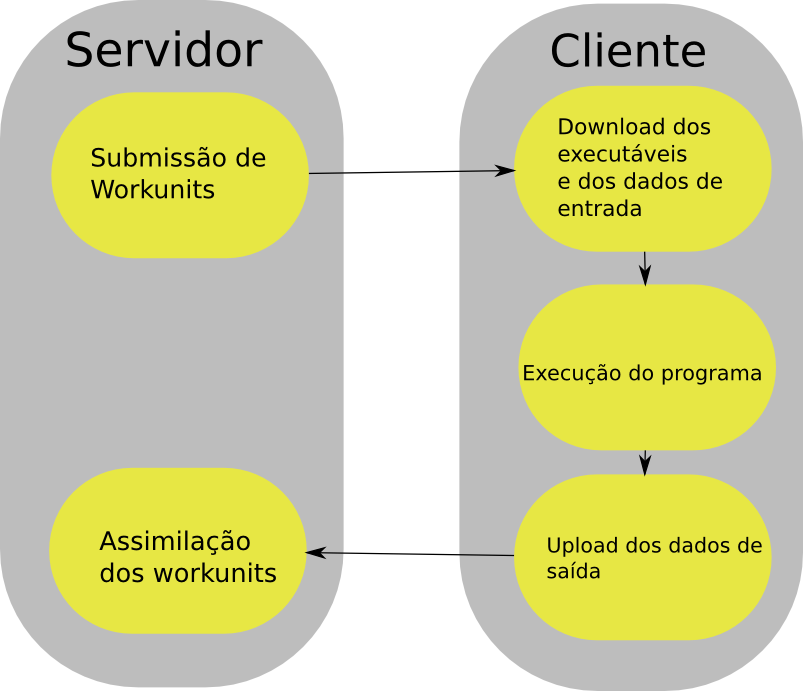
\includegraphics[scale=0.5]{boinc-schema.png}
  \caption{Funcionamento do Boinc}
  \label{funcionamento-boinc}
\end{figure}

\newpage

\subsubsection{Wrapper}


O \emph{Wrapper} é um programa escrito utilizando a \emph{api} do \emph{BOINC}, cujo objetivo é executar aplicações legadas, 
i.e. aplicações que não utilizam a API do \emph{BOINC}, utilizando o \textit{BOINC}. Há uma versão do Wrapper distribuída junto com o 
\textit{BOINC} que utiliza um arquivo XML, mas existe uma outra opção descrita no artigo \cite{hungaro} que utiliza um shell para a 
execução dos aplicativos. Os diagramas de funcionamento do 
\emph{BOINC} com um programa escrito com a api e com o wrapper podem ser vistas nas figuras \ref{boinc-api} e \ref{boinc-wrap} 
respectivamente.


O arquivo XML de execução tem a seguinte estrutura:

\begin{verbatim}
<job_desc>
    <task>
        <application>foobar</application>
        [ <stdin_filename>stdin_file</stdin_filename> ]
        [ <stdout_filename>stdout_file</stdout_filename> ]
        [ <stderr_filename>stderr_file</stderr_filename> ]
        [ <command_line>--foo bar</command_line> ]
    </task>
    [ ... ]
</job_desc>
\end{verbatim}

Neste XML, o único campo obrigatório é o \emph{application}, que é a aplicação
que será executada e pode ser distribuída junto com a aplicação ou já existir no 
computador que o cliente estará instalado (para este segundo caso é necessário
informar o caminho inteiro do executável). É possível ter mais de uma tag
task, e o wrapper as executará sequencialmente. É de responsabilidade
do \textit{Wrapper} perceber se a execução do programa foi feita com sucesso, 
mas não é responsabilidade dele verificar se os pré-requisitos que o programa necessida
estão presentes no sistema. 


\begin{figure}[!h]
  \centering
  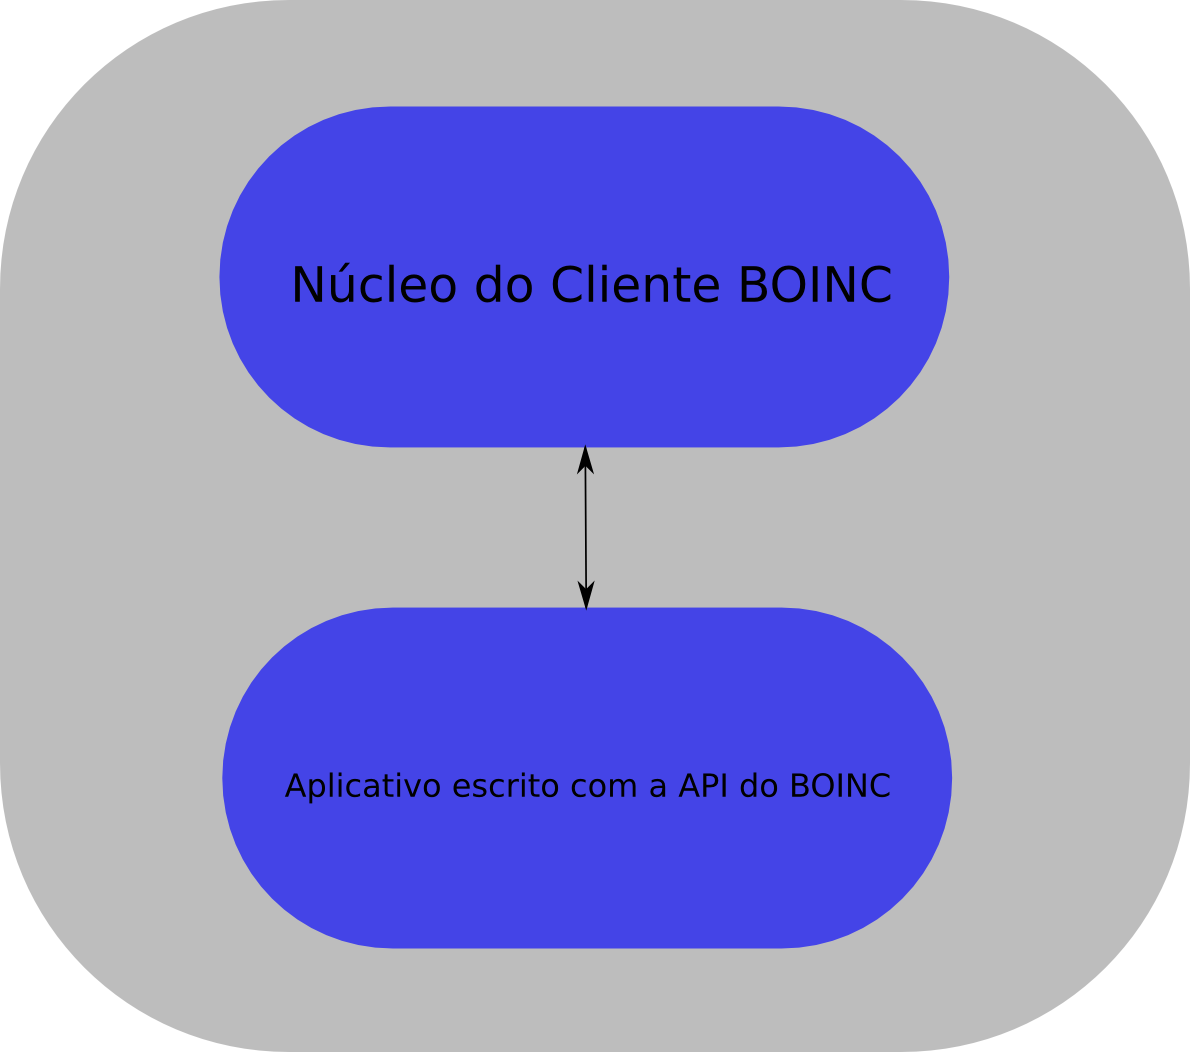
\includegraphics[scale=0.3]{boinc-api.png}
  \caption{Funcionamento do Boinc utilizando uma aplicação que utiliza sua api}
  \label{boinc-api}
\end{figure}


\begin{figure}[!h]
  \centering
  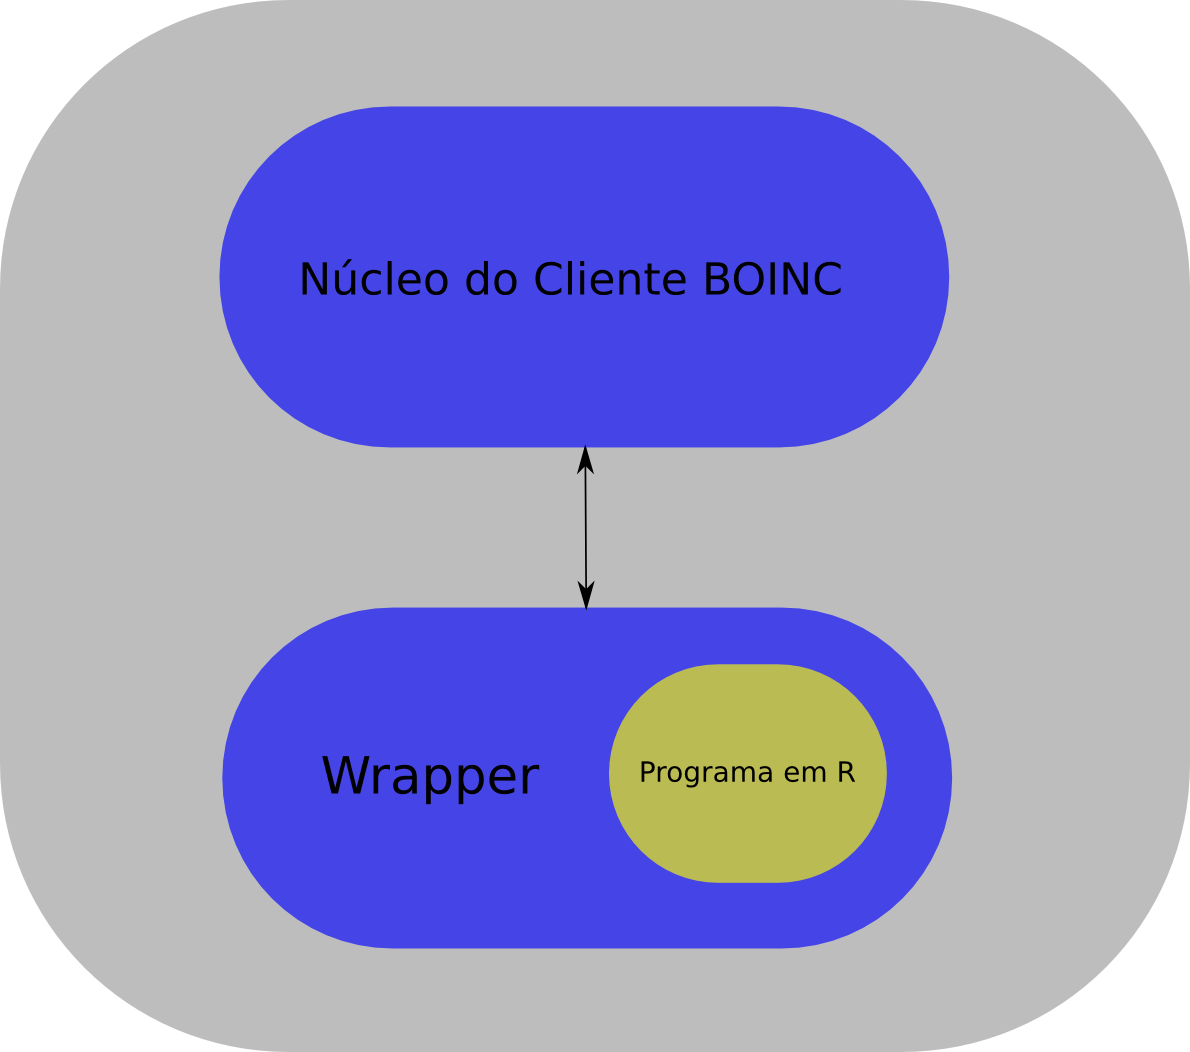
\includegraphics[scale=0.3]{boinc-wrap.png}
  \caption{Funcionamento do Boinc utilizando uma aplicação que utiliza o \emph{wrapper}}
  \label{boinc-wrap}
\end{figure}


\subsection{R}

A linguagem de programação estatística \emph{R} é uma implementação da linguagem \emph{S} e foi criada por Ross Ihaka e Robert
Gentleman na Universidade de Auckland, da Nova Zelândia. A linguagem e ambiente para cálculos estatísticos é considerada
padrão %http://www.nytimes.com/2009/01/07/technology/business-computing/07program.html?_r=1
na área de análise de dados e além do ambiente acadêmico, empresas como \emph{Google}, \emph{Pfizer} e \emph{Merck} a utilizam em seus
processos de mineração de dados. 

Dentre as facilidades que seu uso proporciona, podemos citar as seguintes:

\begin{itemize}
  \item Grande quantidade de funções estatísticas de uso cotidiano na análise de dados
como cálculo de média, desvio padrão, ajuste de curvas, análise de séries temporais. Há também funções mais complexas como por 
exemplo implementações de algoritmos de \emph{clustering}. 
  \item Utilizando o \emph{R} é possível fazer operações em tabelas semelhantes a que normalmente 
são feitas em bancos de dados relacionais como seleção de linhas em tabelas que atendem
certas condições. 
  \item O \emph{R} possui também rotinas de manipulação de matrizes e resolução de sistemas lineares, que são essenciais
em qualquer tarefa de cálculo numérico. 
  \item Gráficos de alta qualidade dos mais variados tipos e para os mais variados propósitos com uma qualidade alta 
também podem ser feitos com o \emph{R}. 
  \item A facilidade de se criar e de se obter pacotes, que nada mais são que conjuntos de rotinas agrupadas, é outro fator
importante: é muito simples criar pacotes e documentá-los. Para disponibilizá-los, pode se submeter um pedido de aprovação 
de para disponibilização no repositório oficial (\url{http://cran-r.c3sl.ufpr.br/})  
do \emph{R}, que possui $2076$ pacotes para os mais diversos fins. O repositório possui \emph{mirrors} espalhados por
todo o mundo, inclusive no Brasil.  
\end{itemize}

Além destes motivos, o artigo \cite{bioconductor} dispõe outros motivos para a utilização do \emph{R} e de seu
pacote para análise de dados de de bioinformática \emph{Bioconductor}.

\begin{itemize}
  \item \textbf{Transparência -} Muitas metodologias de análise na área de biologia e bioinformática computacional
são extremamente complexas e muitas etapas são necessárias na conversão de informação bruta (como por exemplo imagens 
escaneadas de \emph{microarray}). Não se sabe a priori, como as análises podem ser sensíveis a estes fatores, e portanto
trabalhos referenciados na área normalmente expõe todo o processo. O uso de mesmo ambiente e das mesmas facilita bastante
esta transparência;
  \item \textbf{Reprodutibilidade -} Experimentos na área de biologia molecular devem publicar listas de ingredientes
e algoritmos para criar substâncias e processos. Um resultado só pode ser verificado se existir uma obediência a 
um protocolo. Seguindo esta linha, a mineração de dados também deve ser bem descrita e tanto o código fonte 
como os dados nos quais a análise é baseada são normalmente publicados junto com um trabalho nesta área. Utilizar
um mesmo ambiente, que pode ser obtido gratuitamente, para as qualquer plataforma, com pacotes 
facilmente extensíveis também facilita este processo.
  \item \textbf{Eficiência do desenvolvimento -} Se pacote foi por ventura desenvolvido para alguma necessidade, ele pode ser publicado
, melhorado, estudado por outros cientistas, e pode ter seu leque de funcionalidades aumentado caso seu uso siga padrões
de código aberto. Para isso é necessário que esteja bem documentado. Tanto o \emph{R} como o \emph{Bioconductor} são softwares
de código aberto e disfrutam desta qualidade.
  \item \textbf{Prototipagem -} Como o \emph{R} é uma linguagem em um nível mais alto que outras linguagens como \emph{C} ou
\emph{FORTRAN}, programar novas rotinas é bem mais simples. Mesmo não tendo uma execução tão eficiente como em outras
linguagens, pode ser utilizado como protótipo, para depois ser implementado em uma linguagem mais eficiente caso o 
resultado seja bom. 

\end{itemize}

\subsection{Utilização do \emph{R} e do \emph{BOINC}}

Dentre as possibilidades de processamento em grade para a linguagem \emph{R}, escolhemos o \emph{BOINC} para o processamento em grade.
Dentre os motivos, podemos citar:

\begin{itemize}
  \item \textbf{Código aberto -} Ambas as tecnologias são de código aberto e possuem licenças que permitem a utilização das duas
ferramentas para qualquer propósito, além da obtenção gratuita e d possibilidade de estudo do código fonte das duas tecnologias.
Outro ponto forte em comum entre elas é a presença de uma comunidade ativa, com fóruns, listas de discussão e canais de IRC.
  \item \textbf{Multiplataforma -}  
  \item \textbf{Execução inalterada de aplicações escritas em \emph{R} -} Utilizando o \emph{wrapper} é possível executar,
sem precisar alterar um byte do código, programas compilados. Utilizando como programa compilado o interpretador do 
\emph{R}, podemos executar rotinas do \emph{R} em utilizando o \emph{wrapper}. Isso poupa o trabalho de reescrever
códigos já previamente escritos e em funcionamento.
  \item \textbf{Possibilidade de se utilizar pacotes do \emph{R} -} Como o \emph{R} possui uma extensibilidade.
\end{itemize}
